\section{Conclusions and Related Work}\label{SecConcl}

This paper presents the Bytecode Modeling Language (BML). BML allows
one to specify and verify an application directly at the level of
bytecode. Its syntax and semantics are directly inspired by the source
code level specification language JML.  The possibility to reason
direct at the level of bytecode, without relying on a compiler, is of
major importance for guaranteeing the security of applications (for
example in a context of mobile code, where some applications are
written in bytecode directly, to avoid security problems related with
compilation). However, to make such verifications tractable, it is
important that the specification language is intuitive and provides a
sufficient degree of abstraction, without the need to talk too much
about the internal structure of the state (heap, store
\emph{etc.}). BML does exactly this: it is designed to be close to the
source code level specification language JML and provides a high level
of abstraction. It is designed for program verification, and its
semantics supports the development of a verification condition
generator for unstructured code. Moreover, because of its close
connection with JML, it is not too complicated to compile source code
level specification into bytecode level specifications.  The BML
language as we have defined it now, corresponds roughly to JML level
0, \emph{i.e.}\ that part of JML whose semantics is relatively well
understood. However, more advanced constructs of JML can be easily
added to BML, if required.

\begin{figure}[t]
\begin{center}
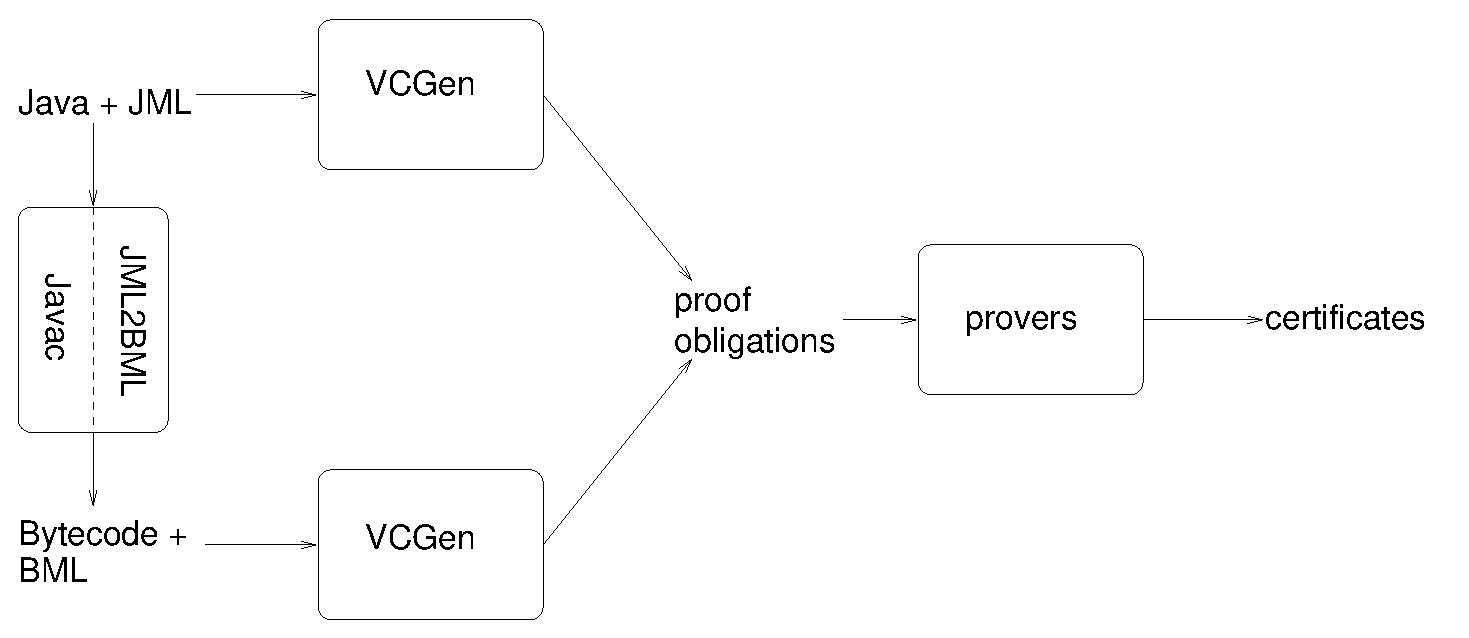
\includegraphics[width=0.8\textwidth]{toolset.eps} 
\vspace*{-1em}
\caption{Overview of \mobius tool set}\label{FigToolSet}
\end{center}
\end{figure}
\paragraph{Tool support}
As part of the \mobius project, we plan to develop a program
verification tool set that supports both JML and
BML. Figure~\ref{FigToolSet} outlines the general architecture of this
tool set. Thus, both Java/JML and bytecode/BML can be used as input
application. Annotated programs are translated into a guarded
command format, for which an appropriate verification condition
generator is used to generate proof obligations that can be discharged
with a theorem prover (either automatic or interactive). To support
the PCC platform, the provers will be instrumented to produce
certificates. In addition, source code applications annotated with JML
can be compiled into bytecode annotated with BML.

The development of the JML subcomponent of the tool set will be based
on experiences with ESC/Java~\cite{CokK04} and JACK~\cite{BurdyRL03}.
Several tools and algorithms (notably the compiler and the
verification condition generator) for BML have already been
implemented, see~\cite{BP06JSV,Pavlova:phd}, but more work is needed
to cover the whole language. Moreover, to make the tool set usable in
practice, we will also need a tool to inspect and write BML
specifications directly, and a run-time checker for BML
specifications. The latter can be implemented by a code
transformation, inserting explicit run-time checks in the bytecode, or
by extending the virtual machine to take the user-specific attributes
with specifications into account.  It is also important to have tool
support for checking the structural and typing constraints for BML
specifications. Such a tool can be built as an extension the Java
bytecode verifier.

Our initial experiments with compilation of specifications has shown
that there exists indeed a correspondence between the proof
obligations generated at source and at bytecode level, modulo
differences in elimination of trivial goals, handling of boolean
expressions, and the naming convention of generated
variables~\cite{Pavlova:phd}. Moreover, when the proofs are done with
the Coq prover, different names are generated for hypotheses at source
code and bytecode level. It is future work to clean up the
compilation, so there is a one-to-one correspondence.




 

\paragraph{Related work}
The interest in specification and verification of bytecode
applications is quite recent, and not too much work has been done in
that direction. Several logics have been developed to reason about
bytecode, \emph{e.g.}~by Bannwart \& M\"uller~\cite{BannwartMueller05}
and within the MRG project~\cite{AspinallEtAl:TPHOLs2004}. However, in
this work the main focus was the development of a sound proof system,
while the focus of BML is to write understandable specifications for
bytecode. JVer is a tool to verify annotated
bytecode~\cite{ChanderEILN05}. However, as specification language they
use a subset of JML, \emph{i.e.}\ a source code level specification language.

The development of BML is clearly inspired by the development of the
JML specification language~\cite{JMLReferenceManual05}. Both JML and
BML follow the Design by Contract principle introduced first in
Eiffel~\cite{Meyer97}. The Boogie project~\cite{BarnettCDJL05}
introduces in similarly the Design by Contract principles into the C\#
programming language, both at source code level and for CIL, the .NET
intermediate language.  The possibility to check a property at
run-time, using the \texttt{assert} construct, has been long 
adopted in the C programming language and recently also in Java (Java
1.5, see \cite[\S 14.10]{JLS}). 

Finally, we should mention the Extended Virtual Platform
project\footnote{See
\url{http://www.cs.usm.maine.edu/~mroyer/xvp/}.}. This project aims at
developing a framework that allows to compile JML annotations, to
allow run-time checking~\cite{AlagicXVP05}. However, in contrast to
our work, they do not intend to do static verification of bytecode
programs. Moreover, their platform takes JML-annotated source code
files as starting point, so it is not possible to annotate bytecode
applications directly.

\vspace*{-.5em}
\subsubsection*{Acknowledgements}
We thank Lennart Beringer and Olha Shkaravska for discussions about
the semantics of BML. 
%\vspace*{-.5em}
